\begin{acquis}
\begin{itemize}
\item BlaBla1
\item BlaBla2
\item BlaBla3
\item BlaBla4
\item BlaBla5
\item BlaBla6
\end{itemize}
\end{acquis}

\QCMautoevaluation{Pour chaque question, plusieurs réponses sont
  proposées.  Déterminer celles qui sont correctes.}

\begin{QCM}
  \begin{GroupeQCM}
  \begin{minipage}[c]{0.44\linewidth}
  Le tableau ci‑contre donne le nombre d'ordinateurs possédés par les familles des élèves de sixième du collège Fontbruant. Il ne concerne que les questions 1 à 3.
   \end{minipage} \hfill%
   \begin{minipage}[c]{0.52\linewidth}
   \begin{center}
    \begin{tabularx}{\linewidth}{|c|X|X|X|X|c|}
    \hline
    Nombre d'ordinateurs & 0 & 1 & 2 & 3 & 4 et plus \\\hline
    Nombre d'élèves & 5 & 19 & 25 & 13 & 8 \\\hline
  \end{tabularx}
   \end{center}
    \end{minipage}\\[1em]
    
    \begin{exercice}
      à quelle(s) question(s) est‑il possible de répondre à l'aide du tableau ?
      \begin{ChoixQCM}{4}
      \item Combien d'élèves de sixième ont un (et un seul) ordinateur ?
      \item Combien d'élèves ont plus de quatre ordinateurs ?
      \item Combien de ces familles sont équipées d'ordinateurs ?
      \item Combien y a‑t‑il d'élèves dans le collège ?
      \end{ChoixQCM}
\begin{corrige}
     \reponseQCM{a} % j'ai mis "a" partout
   \end{corrige}
    \end{exercice}
    
    
    \begin{exercice}
      D'après le tableau, on peut dire que \ldots
      \begin{ChoixQCM}{4}
      \item 24 élèves ont au moins deux ordinateurs
      \item À eux tous, ils ont 145 ordinateurs
      \item 21 élèves ont plus de deux ordinateurs
      \item Il y a 70 élèves en sixième
      \end{ChoixQCM}
\begin{corrige}
     \reponseQCM{a}
   \end{corrige}
    \end{exercice}
    
    
    \begin{exercice}
      Si les ordinateurs étaient répartis équitablement, les élèves auraient environ \ldots
      \begin{ChoixQCM}{4}
      \item 1 ordinateur chacun
      \item 2 ordinateurs chacun 
      \item 3 ordinateurs chacun
      \item 4 ordinateurs chacun
      \end{ChoixQCM}
\begin{corrige}
     \reponseQCM{a}
   \end{corrige}
    \end{exercice}
    
    
    \begin{exercice}
      \begin{center} 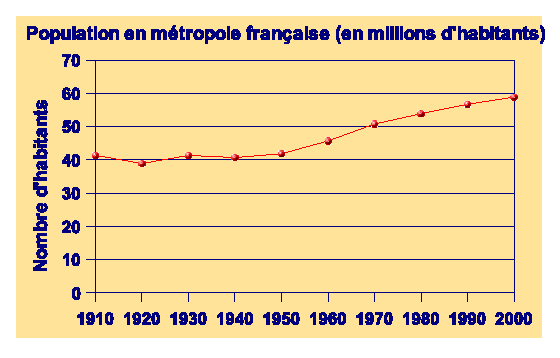
\includegraphics[width=4.4cm]{agmentation_popul} \end{center}
      \begin{ChoixQCM}{4}
      \item La population augmente depuis 1940
      \item La population a atteint 50 millions d'habitants en 1960
      \item Le nombre d'habitants était quasiment le même en 1910 et 1930
      \item Le nombre d'habitants en France métropolitaine est, durant cette période, resté inférieur à 60 millions
      \end{ChoixQCM}
\begin{corrige}
     \reponseQCM{a}
   \end{corrige}
    \end{exercice}
 
 
    \begin{exercice}
      \begin{center} Origine des véhicules situés \end{center}
      \vspace{-0.6cm}
      \begin{center} sur un parking \end{center}
      \begin{center} 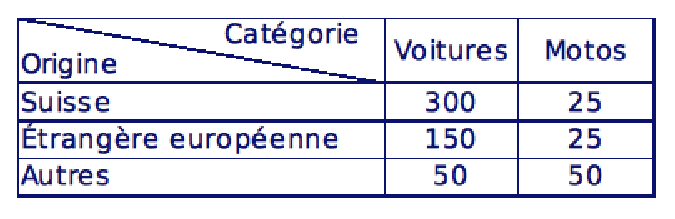
\includegraphics[width=4.5cm]{parking_auto} \end{center}
      \begin{ChoixQCM}{4}
      \item 500 véhicules Suisses sont stationnés sur le parking
      \item La moitié des véhicules sont de nationalité étrangère
      \item Les voitures sont 5 fois plus nombreuses que les motos
      \item 600 personnes ont garé leur véhicule sur le parking
      \end{ChoixQCM}
\begin{corrige}
     \reponseQCM{a}
   \end{corrige}
    \end{exercice}
    

\end{GroupeQCM}
\end{QCM}

  